<<<<<<< HEAD
\chapter{Квазиклассическое приближение}

\section{Критерий применимости квазиклассического приближения}

$\hbar \to 0$ (<<жаргон>>, т.к. физическую константу нельзя устремить к нулю). Принцип соответствия (\textsection\textsection 2,3 гл. 5).

\subsection{Переход к уравнению Гамильтона-Якоби}

$$
i\hbar \pd{}{t} \Psi(\vr, t) = \brcr{-\frac{\hbar^2}{2m} \nabla^2 + U(\vr)} \Psi(\vr,t)
$$
$$
\Psi = \mathcal{A} e^{\frac{i}{\hbar}S(\vr,t)}
$$
где $S \in \mathbb{C}$ имеет размерность действия.

$$
\nabla \Psi(\vr,t) = \brc{\frac{i}{\hbar}\nabla S}\Psi
$$
Подставим $\Psi$ и $\nabla \Psi$ в уравнение Шрёдингера:
$$
i\hbar\brc{\frac{i}{\hbar}\pd{S}{t}}\Psi = 
\brcr{ -\frac{\hbar^2}{2m} \brs{ \brc{\frac{i}{\hbar}\nabla S}^2 + \frac{i}{\hbar}{\nabla^2} S} + U(\vr) } \Psi
$$
\begin{equation}
\label{eq:11_1_1}
\boxed{-\pd{S}{t} = \frac{(\nabla S)^2}{2m} + U(\vr) - \frac{i\hbar}{2m} (\nabla^2 S)}
\end{equation}
Последний член в этом уравнении называется квантовой поправкой.

Мы получили уравнение Гамильтона-Якоби (см. т.1 Л.-Л., \textsection 47):
$$
\begin{gathered}
\boxed{\pd{S}{t} + H(\vr,\vp,t) = 0}\\
H(\vr,\vp,t) = \frac{\vp^2}{2m} + U(\vr) \\
\vp=\nabla S
\end{gathered}
$$

\underbar{Критерий} применимости квазиклассического приближения:
$$
\abs{i\hbar(\nabla^2 S)} \ll \abs{(\nabla S)^2} ~~\rightarrow~~ \frac{\hbar \abs{\nabla^2 S}}{(\nabla S)^2} \ll 1
$$
Подставив $\nabla S =\vp$:
$$
\frac{\hbar}{p^2}\abs{\Div \vp} \ll 1
$$
Или в одномерном случае:
$$
\boxed{\frac{\hbar}{p^2}\abs{\frac{dp}{dx}} \ll 1}
$$
Перепишем критерий в другой форме:
$$
\begin{gathered}
\frac{\hbar}{p^2} \abs{\frac{dp}{dx}} = 
\abs{\frac{d}{dx}\brc{\frac{\hbar}{p}}} _{\text{\eqref{eq:1_1_2}}} = \abs{\frac{d\lambdabar}{dx}} \ll 1\\
\boxed{\Delta \lambdabar \approx \lambdabar \abs{\frac{d\lambdabar}{dx}} \ll \lambdabar}
\end{gathered}
$$
Существует также формальный \underbar{признак} квазиклассичности (т.е. необходимое, но недостаточное условие) (см. т.III Л.Л., \textsection 46):
$$
\boxed{\frac{\lambdabar}{L} \ll 1}
$$
Выразим критерий квазиклассичности через потенциальную энергию:
$$
\frac{p^2(x)}{2m} + U(x) = E ~~\rightarrow~~ p(x)=\sqrt{2m(E-U(x))}
$$
$$
\frac{dp}{dx}=\frac{2m}{2p}\brc{-\frac{dU}{dx}} = \frac{m}{p}F,
$$
где $F$ --- классическая сила.
$$
\boxed{\Delta \lambdabar \ll \lambdabar,~~~\abs{\frac{d\lambdabar}{dx}} \ll 1,~~~\frac{\hbar}{p^2} \abs{\frac{dp}{dx}} \ll 1, ~~~\abs{\frac{\hbar m}{p^3} \frac{dU}{dx}} \ll 1 }
$$
--- критерий квазиклассичности, который удобно использовать при решении задач.

Выводы:
\begin{enumerate}
\item Квазиклассическое приближение не применимо при малых $p$, а также при $p(x)=0$ (классическая точка поворота).
\item В квазиклассическом приближении $U(x)$ не должна иметь резких скачков 
\end{enumerate}

Квазиклассичность = большие импульсы + плавный ход потенциала.

\section{Метод Вентцеля-Крамерса-Бриллюэна (ВКБ)}
\subsection{Вид волновой функции в квазиклассическом приближении}

Раскладывая $S(\vr,t)$ по степеням малого безразмерного параметра, в который входит $\hbar$ (например по $\hbar/pL \sim \lambdabar/L \sim 1/kL \ll 1$), получим:
$$
S(\vr,t)=S_0 + S_1 + S_2 + ...
$$
(обычно будем ограничиваться 1-м порядком)

\begin{figure}
\centering
\begin{tikzpicture}[domain=0:4]
    \draw[->] (-0.1,0) -- (5,0) node[right] {$x$};
    \draw[->] (0,-0.1) -- (0,3) node[above] {$U(x)$};
	\draw [domain=0:4.8, samples=50] plot (\x, {1}) node[right] {$E$};
	\draw [domain=0:2.7, samples=50] plot (\x, {0.2*exp(\x)});
	\draw[dashed] (1.609,3) -- (1.609,0) node[below] {$x_0$};
	\draw (0.8,2.2) node[inner sep=1pt,above,draw,circle] {I};
	\draw (3.5,2.2) node[inner sep=1pt,above,draw,circle] {II};
\end{tikzpicture}
\caption{Классически разрешённая (I) и запрещённая (II) области} \label{fig:1}
\end{figure}

Область применимости метода ВКБ шире, чем классической теории: он работает при $E < U(x)$.

Рассмотрим консервативную систему (см. т.1 Л.-Л., \textsection 47):
$$
S(x,t) = -Et + S(x)
$$
Подставим в \eqref{eq:11_1_1}:
$$
(S')^2 - i\hbar S'' = 2m(E-U(x)) \equiv p^2(x)
$$

Здесь $p^2(x)$ - просто обозначение, которое не подразумевает, что $p^2(x) > 0$.

Разложим $p^2(x)$ до первой степени по $\hbar$:
$$
p^2(x) = (S'_0 + S'_1 + ...)^2 - i\hbar(S''_0+S''_1+...) \approx (S'_0)^2 + 2 S'_0 S'_1 - i\hbar S''_0
$$

Рассмотрим две области на графике:
\renewcommand{\labelenumi}{(\alph{enumi})}
\begin{enumerate}
\item Область I, $p^2(x)>0$

\underbar{Нулевой порядок по $\hbar$}:
$$
\begin{gathered}
(S'_0)^2 = p^2(x) ~~ \rightarrow~~ S'_0 = \mp p(x)\\
\boxed{S_0(x) = \pm \int_x^{x_0} p(x')dx',~ x<x_0}
\end{gathered}
$$
$S_0(x_0)$ здесь отсутствует, так как будет входить в постоянную $\mathcal{A}$.

\underbar{Первый порядок по $\hbar$}:
$$
2 S'_0 S'_1 - i\hbar S''_0 = 0
$$
$$
S'_1 = \frac{i\hbar}{2} \frac{S''_0}{S'_0} = \frac{i\hbar}{2} \brc{\frac{\mp p'(x)}{\mp p(x)}} = \frac{i\hbar}{2} \frac{d}{dx}\brs{\ln p(x)}
$$
$$
S_1 = \frac{i\hbar}{2} \ln p(x) = \boxed{i\hbar \ln \sqrt{p(x)}}
$$
Вид квазиклассической волновой функции в классически разрешённой области:
$$
\boxed{\left. \Psi(x) \right|_{x<x_0} = \mathcal{A} e^{\frac{i}{h} S(x)} \approx \frac{\mathcal{A}}{\sqrt{p(x)}} \exp \brc{\pm\frac{i}{h}\int_x^{x_0} p(x')dx'} }
$$

\item Область II (классически запрещенная), $E<U(x)$, $p^2(x)<0$
$$
p^2(x) = 2m(E-U(x)) = -2m(U(x)-E)
$$
$$
p(x) = \pm i \sqrt{2m(U(x)-E)} = \pm i \abs{p(x)}
$$
Вид квазиклассической волновой функции в классически запрещенной области:
$$
\boxed{\left. \psi(x) \right|_{x>x_0} = \mathcal{A} e^{\frac{i}{h} S(x)} \approx \frac{\mathcal{A}}{\sqrt{\abs{p(x)}}} \exp \brc{\pm\frac{1}{h}\int_{x_0}^{x} \abs{p(x')}dx'} }
$$
\end{enumerate}

Выводы:
\renewcommand{\labelenumi}{\arabic{enumi})}
\begin{enumerate}
\item При $x<x_0$~ $\psi(x) \sim \cos, \sin$\\
При $x>x_0$~ $\psi(x) \sim$ затухающей экспоненте
\item При $p(x_0) = 0$ квазиклассическое приближение не применимо
\item $W(x_0) \sim \frac{1}{p(x_0)} \to \infty$
\end{enumerate}

\begin{excr}
Показать, что волновая функция в областях I и II имеет вид:
$$
\begin{gathered}
\psi_I(x) \simeq \frac{1}{\sqrt{p(x)}} \brcr{a \sin(z+\gamma_1) + b \cos(z+\gamma_2)},~~ z = \frac{1}{h}\int_x^{x_0} p(x')dx'\\
\psi_{II}(x) \simeq \frac{1}{\sqrt{\abs{p(x)}}} \brcr{A e^{-\abs{z}} + B e^{\abs{z}}},~~ \abs{z} = \frac{1}{h}\int_x^{x_0} \abs{p(x')}dx'
\end{gathered}
$$
\end{excr}

\subsection{Связь между двумя решениями, взятыми по разные стороны от точки поворота}
Заменим в окрестности $x_0$ функцию $U(x)$ ее линейным приближением:
$$
\left. U(x) \right|_{\abs{x-x_0} \to 0} \simeq U(x_0) + U'(x_0)(x-x_0)+...
$$

[картинка]

$$
p^2(x) = 2m(E-U(x)) \simeq 2m U'(x_0)(x_0 - x) \equiv \alpha \hbar^2 (x_0 - x)
$$
$$
\psi''(x) + \frac{2m}{\hbar^2} (E-U(x)) \psi(x) = 0 ~~\rightarrow~~ \psi''(x) - \alpha(x-x_0) \psi(x) = 0
$$
$$
\xi = \alpha^{\frac{1}{3}} (x-x_0)
$$
$$
\boxed{
	\frac{d^2}{d\xi^2}\psi(\xi) - \xi\psi(\xi) = 0
}
$$
--- уравнение Эйри (см. \textsection 24, \textsection b, мат. дополнение т.III Л.-Л.)

$$
\left\{
\begin{aligned}
\Ai(\xi) &= \frac{1}{\pi} \int_0^\infty \cos\brs{\xi t + \frac{t^3}{3}} dt \\
\Bi(\xi) &= \frac{1}{\pi} \int_0^\infty \brs{ \sin\brc{\xi t + \frac{t^3}{3}} + \exp\brc{\xi t - \frac{t^3}{3}} } dt
\end{aligned}
\right.
$$

\begin{figure}[h]
\centering
\includegraphics[scale=0.4]{figs/11_2}
\caption{графики функций Эйри}
\label{fig:11_2}
\end{figure}

Асимптотическая область: Эйри + ВКБ приближения.

Эйри-приближение верно при $\abs{x-x_0} < L$, где $L$ --- характерный размер (длина, на которой существенно меняется потенциал).

ВКБ:
$$
\abs{\frac{\hbar m}{p^3} \frac{dU}{dx}} \ll 1
$$
$$
\abs{p^3(x)} \simeq \Bigl( 2m \abs{U'(x_0)} \cdot \abs{x-x_0} \Bigr)^{\frac{3}{2}}
$$
$$
\abs{x-x_0}^{\frac{3}{2}} \gg \frac{\hbar m \abs{U'}}{\brc{2m \abs{U'}}^{3/2}} \sim \frac{\hbar}{\brc{m \abs{U'(x_0)}}^{1/2}}
$$
\begin{equation}
\label{eq:11_2_1}
\abs{x-x_0} \gg \frac{\hbar^{2/3}}{\brc{m \abs{U'(x_0)}}^{1/3}}
\end{equation}

$$
m \abs{U'(x_0)} \sim \left. \frac{p^2(x)}{\abs{x-x_0}} \right|_{\abs{x-x_0} \lesssim L} ~~\rightarrow~~
\Bigl( m\abs{U'(x_0)} \Bigr)^{\frac{1}{3}} \sim \brc{\frac{p^2(x)}{L}}^{\frac{1}{3}}
$$

$$
\left\{
\begin{aligned}
\abs{x-x_0} &\gg \brc{\frac{\hbar}{p(x)}}^{\frac{2}{3}} L^{\frac{1}{3}} = \brc{\frac{\lambdabar}{L}}^{\frac{2}{3}} L\\
\abs{x-x_0} &< L
\end{aligned}
\right.
$$
Эта система совместна только если выполняется условие $\lambdabar/L \ll 1$, то есть:
$$
\boxed{\brc{\frac{\lambdabar}{L}}^{\frac{2}{3}} L \ll \abs{x-x_0} < L} ,~~\text{если}~\frac{\lambdabar}{L} \ll 1
$$

Из \eqref{eq:11_2_1}: $\abs{\xi} \gg 1$. Приведём асимптотические оценки функций Эйри (см. \textsection b, мат. дополнение т.III Л.-Л.)
$$
\left\{
\begin{aligned}
\Ai(\abs{\xi})_{\abs{\xi} \to \infty} &\simeq \frac{1}{2\sqrt{\pi}} \xi^{-\frac{1}{4}} \exp\brc{-\frac{2}{3}\xi^{\frac{3}{2}}} \\
\Bi(\abs{\xi})_{\abs{\xi} \to \infty} &\simeq \frac{1}{\sqrt{\pi}} \xi^{-\frac{1}{4}} \exp\brc{\frac{2}{3}\xi^{\frac{3}{2}}}
\end{aligned}
\right.
~~~
\left\{
\begin{aligned}
\Ai(-\abs{\xi})_{\abs{\xi} \to \infty} &\simeq \frac{1}{\sqrt{\pi}} \abs{\xi}^{-\frac{1}{4}} \sin\brs{\frac{2}{3} \abs{\xi}^{\frac{3}{2}} + \frac{\pi}{4}} \\
\Bi(-\abs{\xi})_{\abs{\xi} \to \infty} &\simeq \frac{1}{\sqrt{\pi}} \abs{\xi}^{-\frac{1}{4}} \cos\brs{\frac{2}{3} \abs{\xi}^{\frac{3}{2}} + \frac{\pi}{4}}
\end{aligned}
\right.
$$

$$
\begin{aligned}
z_{(x \to x_0 - 0)} &\to \frac{1}{\hbar} \int_{x}^{x_0} \alpha^{\frac{1}{2}}\hbar(x_0-x')^{\frac{1}{2}} dx' = \frac{2}{3}\alpha^{\frac{1}{2}} (x_0-x')^{\frac{3}{2}} \equiv \frac{2}{3}\alpha^{\frac{1}{2}} \abs{x-x_0}^{\frac{3}{2}} \equiv \frac{2}{3} \abs{\xi}^{\frac{3}{2}} \\
z_{(x \to x_0 + 0)} &\to \frac{1}{\hbar} \int_{x_0}^{x} \alpha^{\frac{1}{2}}\hbar(x'-x_0)^{\frac{1}{2}} dx' = ... = \frac{2}{3} \xi^{\frac{3}{2}}
\end{aligned}
$$

$$
\begin{aligned}
\left. \psi_{I}(x) \right|_{x<x_0}
&\xrightarrow{\text{ВКБ}} \left. \frac{1}{\sqrt{p}} \brcr{a \sin[z+\gamma_1] + b \cos[z+\gamma_2]} \right|_{(x \to x_0 - 0)} =\\
&= \frac{1}{\alpha^{\frac{1}{6}} \hbar^{\frac{1}{2}} \abs{\xi}^{\frac{1}{4}}} \brcr{a \sin\brs{\frac{2}{3}\abs{\xi}^{\frac{3}{2}} + \gamma_1} + b \cos\brs{\frac{2}{3}\abs{\xi}^{\frac{3}{2}}+ \gamma_2} }
\end{aligned}
$$

$$
\left. \psi_{II}(x) \right|_{x>x_0} \xrightarrow{\text{ВКБ}} \left. \frac{1}{\sqrt{p}} \brcr{A e^{-\abs{z}} + B e^{\abs{z}}} \right|_{(x \to x_0 + 0)} =
\frac{1}{\alpha^{\frac{1}{6}} \hbar^{\frac{1}{2}} \xi^{\frac{1}{4}}} \brcr{A \exp\brc{-\frac{2}{3}\xi^{\frac{3}{2}}} + B \exp\brc{\frac{2}{3}\xi^{\frac{3}{2}}}}
$$

Сравнивая с асимптотическими оценками, пролучаем значения констант:
$$
\begin{gathered}
\gamma_1 = \gamma_2 = \frac{\pi}{4}\\
\frac{A}{a} = \frac{1}{2},~ \frac{B}{b} = 1 ~~\rightarrow~~ \boxed{A = \frac{a}{2},~ B = b}
\end{gathered}
$$

Общее решение:
$$
\begin{aligned}
\psi_{I}(x) &\simeq \frac{1}{\sqrt{p(x)}} \brcr{ a \sin\brs{\frac{1}{\hbar} \int_x^{x_0} p(x')dx'+\frac{\pi}{4}} + b \cos\brs{\frac{1}{\hbar} \int_x^{x_0} p(x')dx'+\frac{\pi}{4}} } \\
\psi_{II}(x) &\simeq \frac{1}{\sqrt{\abs{p(x)}}} \brcr{ \frac{a}{2} \exp\brc{-\frac{1}{\hbar} \int^x_{x_0} \abs{p(x')}dx'} + b \exp\brc{-\frac{1}{\hbar} \int^x_{x_0} \abs{p(x')}dx'} }
\end{aligned}
$$

\textbf{Правило I:} \\
$B = b = 0$, $\Ai(\abs{\xi})_{\abs{\xi} \to \infty}$
$$
\boxed{
	\psi(x)_{(x \gg x_0)} = \frac{a}{2 \sqrt{\abs{p}}} \exp\brc{-\frac{1}{\hbar} \int_{x_0}^{x} \abs{p(x')}dx'} ~~\rightarrow~~
	\psi(x)_{(x \ll x_0)} = \frac{a}{\sqrt{p}} \sin\brc{\frac{1}{\hbar} \int_{x}^{x_0} p(x')dx' + \frac{\pi}{4}}
}
$$
В обратную сторону данный переход не будет корректным.
\\

\textbf{Правило II:} \\
$\phi$ --- поправка от приближения
$$
\begin{aligned}
\psi(x)_{(x \ll x_0)} = \frac{c}{\sqrt{p}} \brcr{\sin\brc{z+\frac{\pi}{4}+\phi}} &\equiv
\frac{c}{\sqrt{p}} \brcr{\sin\brc{z+\frac{\pi}{4}}\cos{\phi} + \cos\brc{z+\frac{\pi}{4}}\sin{\phi}} =\\
&=\frac{1}{\sqrt{p}} \brcr{a \sin\brc{z+\frac{\pi}{4}} + b \cos\brc{z+\frac{\pi}{4}}}
\end{aligned}
$$
где $c\sin{\phi}=b$, $c\cos{\phi}=a$

$$
\boxed{
	\psi(x)_{(x \ll x_0)} = \frac{c}{\sqrt{p}} \sin\brc{\frac{1}{\hbar} \int_{x}^{x_0} p(x')dx' + \frac{\pi}{4} + \phi} ~~\rightarrow~~
	\psi(x)_{(x \gg x_0)} = \frac{c \sin{\phi}}{\sqrt{\abs{p}}} \exp\brc{\frac{1}{\hbar} \int_{x_0}^{x} \abs{p(x')}dx'}
}
$$
Переход не работает, когда $\psi \to \pi n$, а также в обратную сторону.

\textbf{Правило III:} \\
Сделаем замену в II: $\phi \to \phi + \frac{\pi}{2}$:
$$
\frac{c}{\sqrt{p}}\cos\brs{z+\frac{\pi}{4} + \phi} ~~\rightarrow~~ \frac{c\cos{\phi}}{\sqrt{\abs{p}}} e^{\abs{z}}
$$

Домножим (II) на $\pm i$ и сложим с предыдущим результатом:
$$
\frac{c}{\sqrt{p}} e^{\pm i\brc{z+\frac{\pi}{4}+\phi}} = \frac{c}{\sqrt{p}} e^{\pm i \phi} e^{\pm i\brc{z+\frac{\pi}{4}}} ~~\rightarrow~~
\frac{c}{\sqrt{\abs{p}}} e^{\pm i \phi} e^{\abs{z}}
$$

$$
\boxed{
\begin{aligned}
	\psi(x)_{(x \ll x_0)} = \frac{C}{\sqrt{p}} \exp\brc{\frac{i}{\hbar} \int_{x}^{x_0} p(x')dx' + \frac{i\pi}{4}} 
	+ \frac{D}{\sqrt{p}} \exp\brc{-\frac{i}{\hbar} \int_{x}^{x_0} p(x')dx' - \frac{i\pi}{4}} ~~\rightarrow~~ \\
	~~\rightarrow~~ \psi(x)_{(x \gg x_0)} = \frac{C+D}{\sqrt{\abs{p}}} \exp\brc{\frac{1}{\hbar} \int_{x_0}^{x} \abs{p(x')}dx'}
\end{aligned}
}
$$

Поменяем области местами. Что произойдёт с правилами сответствия? Если грубо, то $x_0$ поменяется местами с $x$ в пределах интегрирования и отношениях типа $\ll$.


\section{Условие квантования Бора-Зоммерфильда}

\begin{figure}[h]
\centering
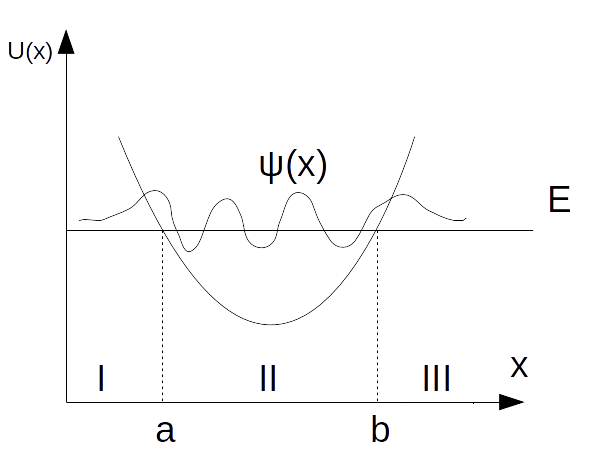
\includegraphics[scale=1]{figs/11_4}
\caption{К выводу условий квантования Бора-Зоммерфельда}
\label{fig:11_4}
\end{figure}

Применим правило соответствия I:
$$
\begin{gathered}
\psi(x)_{x<b} = \frac{a_1}{\sqrt{p}} \sin\brs{\frac{1}{\hbar} \int_{x}^{b} p(x')dx' + \frac{\pi}{4} } \equiv \frac{a_1}{\sqrt{p}} \sin({z_1 + \frac{\pi}{4}}) \\
\psi(x)_{x>a} = \frac{a_2}{\sqrt{p}} \sin\brs{\frac{1}{\hbar} \int_{a}^{x} p(x')dx' + \frac{\pi}{4} } \equiv \frac{a_2}{\sqrt{p}} \sin({z_2 + \frac{\pi}{4}})
\end{gathered}
$$
$$
z_1+z_2 = \frac{1}{\hbar} \int_{a}^{b} p(x')dx' \equiv \frac{1}{\hbar} \int_{a}^{b} p(x)dx
$$
<<Сшивка>> (на интервале $(a, b)$ волновые функции обязаны совпадать):
$$
\begin{aligned}
\frac{a_1}{\sqrt{p}} \sin({z_1+\frac{\pi}{4}}) = \frac{a_2}{\sqrt{p}} \sin({z_2+\frac{\pi}{4}}) = \frac{a_2}{\sqrt{p}} \sin\brs{\frac{1}{\hbar} \int_{a}^{b} p(x)dx - z_1 + \frac{\pi}{4}} = \\
= -\frac{a_2}{\sqrt{p}} \sin\brs{z_1 - \frac{1}{\hbar} \int_{a}^{b} p(x)dx - \frac{\pi}{4} }
\end{aligned}
$$

Условия совпадения решений:
\begin{equation}
\label{eq:11_3_1}
z_1 + \frac{\pi}{4} = z_1 - \frac{1}{\hbar} \int_{a}^{b} p(x)dx - \frac{\pi}{4} + \pi(n+1) \\
\end{equation}
\begin{equation}
\label{eq:11_3_2}
a_1 = (-1)(-1)^{n+1}a_2  ~~\rightarrow~~ a_2 = a_1 (-1)^n
\end{equation}

Отсюда получаем \textbf{условия квантования Бора-Зоммерфильда} (1915-й год):
\begin{equation}
\label{eq:11_3_3}
\boxed{\int_{a}^{b} p(x)dx = \pi\hbar\brc{n+\frac{1}{2}}}
\end{equation}

\begin{equation}
\label{eq:11_3_4}
\boxed{\oint p(x)dx \equiv \int_{a}^{b} p(x)dx = 2\pi\hbar\brc{n+\frac{1}{2}}}
\end{equation}

Напомним:
$$
p(x) = \sqrt{2m(E_n - U(x))}
$$

Выводы:
\begin{enumerate}
\item $\oint p(x)dx $ --- адиабатический инвариант (система сохраняет квантовый уровень при медленном (адиабатическом) изменении параметров системы)
\item $n:~ n \to E_n$
$$
\sin({z+\frac{\pi}{4}}):~~ a \to b:~ \frac{\pi}{4} \to \frac{1}{\hbar} \left. \int_{a}^{b} p(x)dx + \frac{\pi}{4} \right|_{\text{\eqref{eq:11_3_3}}} =
\pi n + \frac{3}{4}\pi
$$
Следовательно, волновая функция на промежутке от $a$ до $b$ меняет знак $n$ раз, что является частным случаем осцилляционной теоремы (гл. 7 \textsection 3)
\end{enumerate}

Малый параметр ВКБ:
$$
\frac{\lambdabar}{L} \sim \frac{1}{n} \ll 1 \sim \frac{1}{2} ~~\rightarrow~~ n >> 1
$$
т.е. условия квантования Бора-Зоммерфильда пригодны при больших $n$ (\textbf{TODO}: почему при этом нельзя опустить $\frac{1}{2}$?)

\section{Фазовый объём, приходящийся на одно квантовое состояние}

Рассмотрим фазовую плоскость $(p,x)$:

$$
\oint p(x)dx = \Gamma(E_n) = 2\pi\hbar\brs{n+\frac{1}{2}}
$$

$$
E_n \to E_{n+1}: \boxed{\Delta\Gamma = \Gamma(E_{n+1}) - \Gamma(E_n) = 2\pi\hbar}
$$
т.е. на одно квантовое состояние в фазовом пространстве частицы приходится объём $2\pi\hbar$

Число квантовых состояний в некотором фазовом объёме:
$$
\boxed{\Delta N = \frac{\Delta p \Delta x}{2\pi\hbar}}
$$

\begin{sloppypar}
  \section{Вероятность проникновения частицы через барьер в квазиклассическом приближении}
\end{sloppypar}

\begin{figure}[h]
\centering
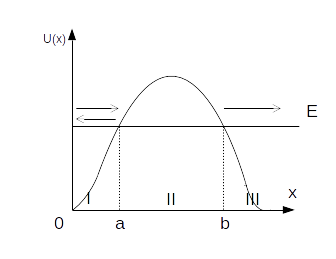
\includegraphics[scale=1]{figs/11_5}
\caption{Проникновение частицы через барьер}
\label{fig:11_5}
\end{figure}


\begin{enumerate}
\item Область III:
$$
\psi(x)_{x>b} \simeq \frac{A}{\sqrt{p(x)}} \exp\brc{\frac{i}{\hbar} \int_{b}^{x} p(x')dx' + i\frac{\pi}{4}}
$$

Проверим, что данная волновая функция действительно соответствует прошедшей волне: найдём плотность потока вероятности:
$$
\begin{aligned}
j_{x}^{\text{прош}} = \frac{i\hbar}{2m}(\psi\nabla\psi^* - \psi^*\nabla\psi) = \brc{\text{члены}~ \sim \nabla \frac{1}{\sqrt{p(x)}} ~\text{компенсируются}} =\\
= \frac{i\hbar}{2m} \brcr{\frac{A}{\sqrt{p(x)}} e^{i\brs{z(x)+\frac{\pi}{4}}} \frac{A^*}{\sqrt{p(x)}} e^{-i\brs{z(x)+\frac{\pi}{4}}} \brc{-i\frac{dz}{dx}} - \brc{\text{компл-сопр}} } = \\
= \frac{i\hbar}{2m} \brcr{\frac{-i\abs{A}^2 2}{\hbar}} = \frac{\abs{A}^2}{m} = j_x^{\text{прош}} > 0
\end{aligned}
$$
т.е. $\psi(x)_{x>b}$ действительно описывает прошедшую волну.

\item Область II, по правилу соответствия III:
$$
\psi(x)_{a<x<b} \simeq \frac{A}{\sqrt{\abs{p}}} \exp\brc{\frac{1}{\hbar} \int_x^{b} \abs{p(x')}dx'} \equiv 
$$
$$
\equiv \frac{A}{\sqrt{\abs{p}}} \underbrace{ \exp\brc{\frac{1}{\hbar} \int_{a}^{b} \abs{p(x')}dx'} }_{e^{\gamma}} \exp\brc{- \frac{1}{\hbar} \int_{a}^{x} \abs{p(x')}dx'}
$$

\item Область I, правило соответствия I:
$$
\psi(x)_{x<a} \simeq \frac{2A}{\sqrt{p}} \sin\brs{\frac{1}{\hbar} \int_{x}^{a} p(x')dx' + \frac{\pi}{4}} e^{\gamma} =
$$
$$
= \frac{2A e^{\gamma}}{\sqrt{p}} \left\{ \underbrace{\exp \brc{\frac{i}{\hbar} \int_{x}^{a} p(x')dx' + \frac{i\pi}{4}}}_{\text{отраженная волна}} - \underbrace{\exp \brc{-\frac{i}{\hbar} \int_{x}^{a} p(x')dx' - \frac{i\pi}{4}}}_{\text{падающая волна}}\right \} 
$$
$$
j_x^{\text{пад}} = \frac{i \hbar}{2m} \brcr{\Psi \nabla \Psi^* - \Psi^* \nabla \Psi} = \frac{i \hbar}{2m} \brcr{\frac{A e^{\gamma}}{i \sqrt{p}} e^{-i(z(x) + \frac{\pi}{4})} \frac{A^* e^{\gamma}}{(-i) \sqrt{p}} e^{i(z(x) + \frac{\pi}{4})} \brc{i \frac{dz}{dx}} - \text{К.С.} } =
$$
$$
= \frac{i \hbar}{2m} \brcr{\frac{-2i \abs{A}^2 e^{2\gamma}}{\hbar}} = \frac{\abs{A}^2 e^{2\gamma}}{m}
$$

\item Формула Гамова (1928г):
$$
\boxed{D \equiv \frac{\abs{j_x^{\text{прош}}}} {\abs{j_x^{\text{пад}}}} = e^{2\gamma} = e^{-\frac{2}{\hbar} \int_a^b \abs{p(x)} dx}} 
$$

Коэффициент отражения:
$$
R \equiv \frac{\abs{j_x^{\text{отр}}}}{\abs{j_x^{\text{пад}}}} = 1 (!)
$$
Это свойство имеет место в квазиклассике, т.к. при установлении правил соответствия растущая экспонента компенсирует падающую экспоненту.

$D \ll 1 \to 2\gamma \ll 1$
\end{enumerate}
=======
\chapter{Квазиклассическое приближение}

\section{Критерий применимости квазиклассического приближения}

$\hbar \to 0$ (<<жаргон>>, т.к. физическую константу нельзя устремить к нулю). Принцип соответствия (\textsection\textsection 2,3 гл. 5).

\subsection{Переход к уравнению Гамильтона-Якоби}

$$
i\hbar \pd{}{t} \Psi(\vr, t) = \brcr{-\frac{\hbar^2}{2m} \nabla^2 + U(\vr)} \Psi(\vr,t)
$$
$$
\Psi = \mathcal{A} e^{\frac{i}{\hbar}S(\vr,t)}
$$
где $S \in \mathbb{C}$ имеет размерность действия.

$$
\nabla \Psi(\vr,t) = \brc{\frac{i}{\hbar}\nabla S}\Psi
$$
Подставим $\Psi$ и $\nabla \Psi$ в уравнение Шрёдингера:
$$
i\hbar\brc{\frac{i}{\hbar}\pd{S}{t}}\Psi = 
\brcr{ -\frac{\hbar^2}{2m} \brs{ \brc{\frac{i}{\hbar}\nabla S}^2 + \frac{i}{\hbar}{\nabla^2} S} + U(\vr) } \Psi
$$
\begin{equation}
\label{eq:11_1_1}
\boxed{-\pd{S}{t} = \frac{(\nabla S)^2}{2m} + U(\vr) - \frac{i\hbar}{2m} (\nabla^2 S)}
\end{equation}
Последний член в этом уравнении называется квантовой поправкой.

Мы получили уравнение Гамильтона-Якоби (см. т.1 Л.-Л., \textsection 47):
$$
\begin{gathered}
\boxed{\pd{S}{t} + H(\vr,\vp,t) = 0}\\
H(\vr,\vp,t) = \frac{\vp^2}{2m} + U(\vr) \\
\vp=\nabla S
\end{gathered}
$$

\underbar{Критерий} применимости квазиклассического приближения:
$$
\abs{i\hbar(\nabla^2 S)} \ll \abs{(\nabla S)^2} ~~\rightarrow~~ \frac{\hbar \abs{\nabla^2 S}}{(\nabla S)^2} \ll 1
$$
Подставив $\nabla S =\vp$:
$$
\frac{\hbar}{p^2}\abs{\Div \vp} \ll 1
$$
Или в одномерном случае:
$$
\boxed{\frac{\hbar}{p^2}\abs{\frac{dp}{dx}} \ll 1}
$$
Перепишем критерий в другой форме:
$$
\begin{gathered}
\frac{\hbar}{p^2} \abs{\frac{dp}{dx}} = 
\abs{\frac{d}{dx}\brc{\frac{\hbar}{p}}} _{\text{\eqref{eq:1_1_2}}} = \abs{\frac{d\lambdabar}{dx}} \ll 1\\
\boxed{\Delta \lambdabar \approx \lambdabar \abs{\frac{d\lambdabar}{dx}} \ll \lambdabar}
\end{gathered}
$$
Существует также формальный \underbar{признак} квазиклассичности (т.е. необходимое, но недостаточное условие) (см. т.III Л.Л., \textsection 46):
$$
\boxed{\frac{\lambdabar}{L} \ll 1}
$$
Выразим критерий квазиклассичности через потенциальную энергию:
$$
\frac{p^2(x)}{2m} + U(x) = E ~~\rightarrow~~ p(x)=\sqrt{2m(E-U(x))}
$$
$$
\frac{dp}{dx}=\frac{2m}{2p}\brc{-\frac{dU}{dx}} = \frac{m}{p}F,
$$
где $F$ --- классическая сила.
$$
\boxed{\Delta \lambdabar \ll \lambdabar,~~~\abs{\frac{d\lambdabar}{dx}} \ll 1,~~~\frac{\hbar}{p^2} \abs{\frac{dp}{dx}} \ll 1, ~~~\abs{\frac{\hbar m}{p^3} \frac{dU}{dx}} \ll 1 }
$$
--- критерий квазиклассичности, который удобно использовать при решении задач.

Выводы:
\begin{enumerate}
\item Квазиклассическое приближение не применимо при малых $p$, а также при $p(x)=0$ (классическая точка поворота).
\item В квазиклассическом приближении $U(x)$ не должна иметь резких скачков 
\end{enumerate}

Квазиклассичность = большие импульсы + плавный ход потенциала.

\section{Метод Вентцеля-Крамерса-Бриллюэна (ВКБ)}
\subsection{Вид волновой функции в квазиклассическом приближении}

Раскладывая $S(\vr,t)$ по степеням малого безразмерного параметра, в который входит $\hbar$ (например по $\hbar/pL \sim \lambdabar/L \sim 1/kL \ll 1$), получим:
$$
S(\vr,t)=S_0 + S_1 + S_2 + ...
$$
(обычно будем ограничиваться 1-м порядком)

\begin{figure}
\centering
\begin{tikzpicture}[domain=0:4]
    \draw[->] (-0.1,0) -- (5,0) node[right] {$x$};
    \draw[->] (0,-0.1) -- (0,3) node[above] {$U(x)$};
	\draw [domain=0:4.8, samples=50] plot (\x, {1}) node[right] {$E$};
	\draw [domain=0:2.7, samples=50] plot (\x, {0.2*exp(\x)});
	\draw[dashed] (1.609,3) -- (1.609,0) node[below] {$x_0$};
	\draw (0.8,2.2) node[inner sep=1pt,above,draw,circle] {I};
	\draw (3.5,2.2) node[inner sep=1pt,above,draw,circle] {II};
\end{tikzpicture}
\caption{Классически разрешённая (I) и запрещённая (II) области} \label{fig:1}
\end{figure}

Область применимости метода ВКБ шире, чем классической теории: он работает при $E < U(x)$.

Рассмотрим консервативную систему (см. т.1 Л.-Л., \textsection 47):
$$
S(x,t) = -Et + S(x)
$$
Подставим в \eqref{eq:11_1_1}:
$$
(S')^2 - i\hbar S'' = 2m(E-U(x)) \equiv p^2(x)
$$

Здесь $p^2(x)$ - просто обозначение, которое не подразумевает, что $p^2(x) > 0$.

Разложим $p^2(x)$ до первой степени по $\hbar$:
$$
p^2(x) = (S'_0 + S'_1 + ...)^2 - i\hbar(S''_0+S''_1+...) \approx (S'_0)^2 + 2 S'_0 S'_1 - i\hbar S''_0
$$

Рассмотрим две области на графике:
\renewcommand{\labelenumi}{(\alph{enumi})}
\begin{enumerate}
\item Область I, $p^2(x)>0$

\underbar{Нулевой порядок по $\hbar$}:
$$
\begin{gathered}
(S'_0)^2 = p^2(x) ~~ \rightarrow~~ S'_0 = \mp p(x)\\
\boxed{S_0(x) = \pm \int_x^{x_0} p(x')dx',~ x<x_0}
\end{gathered}
$$
$S_0(x_0)$ здесь отсутствует, так как будет входить в постоянную $\mathcal{A}$.

\underbar{Первый порядок по $\hbar$}:
$$
2 S'_0 S'_1 - i\hbar S''_0 = 0
$$
$$
S'_1 = \frac{i\hbar}{2} \frac{S''_0}{S'_0} = \frac{i\hbar}{2} \brc{\frac{\mp p'(x)}{\mp p(x)}} = \frac{i\hbar}{2} \frac{d}{dx}\brs{\ln p(x)}
$$
$$
S_1 = \frac{i\hbar}{2} \ln p(x) = \boxed{i\hbar \ln \sqrt{p(x)}}
$$
Вид квазиклассической волновой функции в классически разрешённой области:
$$
\boxed{\left. \Psi(x) \right|_{x<x_0} = \mathcal{A} e^{\frac{i}{h} S(x)} \approx \frac{\mathcal{A}}{\sqrt{p(x)}} \exp \brc{\pm\frac{i}{h}\int_x^{x_0} p(x')dx'} }
$$

\item Область II (классически запрещенная), $E<U(x)$, $p^2(x)<0$
$$
p^2(x) = 2m(E-U(x)) = -2m(U(x)-E)
$$
$$
p(x) = \pm i \sqrt{2m(U(x)-E)} = \pm i \abs{p(x)}
$$
Вид квазиклассической волновой функции в классически запрещенной области:
$$
\boxed{\left. \psi(x) \right|_{x>x_0} = \mathcal{A} e^{\frac{i}{h} S(x)} \approx \frac{\mathcal{A}}{\sqrt{\abs{p(x)}}} \exp \brc{\pm\frac{1}{h}\int_{x_0}^{x} \abs{p(x')}dx'} }
$$
\end{enumerate}

Выводы:
\renewcommand{\labelenumi}{\arabic{enumi})}
\begin{enumerate}
\item При $x<x_0$~ $\psi(x) \sim \cos, \sin$\\
При $x>x_0$~ $\psi(x) \sim$ затухающей экспоненте
\item При $p(x_0) = 0$ квазиклассическое приближение не применимо
\item $W(x_0) \sim \frac{1}{p(x_0)} \to \infty$
\end{enumerate}

\begin{excr}
Показать, что волновая функция в областях I и II имеет вид:
$$
\begin{gathered}
\psi_I(x) \simeq \frac{1}{\sqrt{p(x)}} \brcr{a \sin(z+\gamma_1) + b \cos(z+\gamma_2)},~~ z = \frac{1}{h}\int_x^{x_0} p(x')dx'\\
\psi_{II}(x) \simeq \frac{1}{\sqrt{\abs{p(x)}}} \brcr{A e^{-\abs{z}} + B e^{\abs{z}}},~~ \abs{z} = \frac{1}{h}\int_x^{x_0} \abs{p(x')}dx'
\end{gathered}
$$
\end{excr}

\subsection{Связь между двумя решениями, взятыми по разные стороны от точки поворота}
Заменим в окрестности $x_0$ функцию $U(x)$ ее линейным приближением:
$$
\left. U(x) \right|_{\abs{x-x_0} \to 0} \simeq U(x_0) + U'(x_0)(x-x_0)+...
$$

[картинка]

$$
p^2(x) = 2m(E-U(x)) \simeq 2m U'(x_0)(x_0 - x) \equiv \alpha \hbar^2 (x_0 - x)
$$
$$
\psi''(x) + \frac{2m}{\hbar^2} (E-U(x)) \psi(x) = 0 ~~\rightarrow~~ \psi''(x) - \alpha(x-x_0) \psi(x) = 0
$$
$$
\xi = \alpha^{\frac{1}{3}} (x-x_0)
$$
$$
\boxed{
	\frac{d^2}{d\xi^2}\psi(\xi) - \xi\psi(\xi) = 0
}
$$
--- уравнение Эйри (см. \textsection 24, \textsection b, мат. дополнение т.III Л.-Л.)

$$
\left\{
\begin{aligned}
\Ai(\xi) &= \frac{1}{\pi} \int_0^\infty \cos\brs{\xi t + \frac{t^3}{3}} dt \\
\Bi(\xi) &= \frac{1}{\pi} \int_0^\infty \brs{ \sin\brc{\xi t + \frac{t^3}{3}} + \exp\brc{\xi t - \frac{t^3}{3}} } dt
\end{aligned}
\right.
$$

\begin{figure}[h]
\centering
\includegraphics[scale=0.4]{figs/11_2}
\caption{графики функций Эйри}
\label{fig:11_2}
\end{figure}

Асимптотическая область: Эйри + ВКБ приближения.

Эйри-приближение верно при $\abs{x-x_0} < L$, где $L$ --- характерный размер (длина, на которой существенно меняется потенциал).

ВКБ:
$$
\abs{\frac{\hbar m}{p^3} \frac{dU}{dx}} \ll 1
$$
$$
\abs{p^3(x)} \simeq \Bigl( 2m \abs{U'(x_0)} \cdot \abs{x-x_0} \Bigr)^{\frac{3}{2}}
$$
$$
\abs{x-x_0}^{\frac{3}{2}} \gg \frac{\hbar m \abs{U'}}{\brc{2m \abs{U'}}^{3/2}} \sim \frac{\hbar}{\brc{m \abs{U'(x_0)}}^{1/2}}
$$
\begin{equation}
\label{eq:11_2_1}
\abs{x-x_0} \gg \frac{\hbar^{2/3}}{\brc{m \abs{U'(x_0)}}^{1/3}}
\end{equation}

$$
m \abs{U'(x_0)} \sim \left. \frac{p^2(x)}{\abs{x-x_0}} \right|_{\abs{x-x_0} \lesssim L} ~~\rightarrow~~
\Bigl( m\abs{U'(x_0)} \Bigr)^{\frac{1}{3}} \sim \brc{\frac{p^2(x)}{L}}^{\frac{1}{3}}
$$

$$
\left\{
\begin{aligned}
\abs{x-x_0} &\gg \brc{\frac{\hbar}{p(x)}}^{\frac{2}{3}} L^{\frac{1}{3}} = \brc{\frac{\lambdabar}{L}}^{\frac{2}{3}} L\\
\abs{x-x_0} &< L
\end{aligned}
\right.
$$
Эта система совместна только если выполняется условие $\lambdabar/L \ll 1$, то есть:
$$
\boxed{\brc{\frac{\lambdabar}{L}}^{\frac{2}{3}} L \ll \abs{x-x_0} < L} ,~~\text{если}~\frac{\lambdabar}{L} \ll 1
$$

Из \eqref{eq:11_2_1}: $\abs{\xi} \gg 1$. Приведём асимптотические оценки функций Эйри (см. \textsection b, мат. дополнение т.III Л.-Л.)
$$
\left\{
\begin{aligned}
\Ai(\abs{\xi})_{\abs{\xi} \to \infty} &\simeq \frac{1}{2\sqrt{\pi}} \xi^{-\frac{1}{4}} \exp\brc{-\frac{2}{3}\xi^{\frac{3}{2}}} \\
\Bi(\abs{\xi})_{\abs{\xi} \to \infty} &\simeq \frac{1}{\sqrt{\pi}} \xi^{-\frac{1}{4}} \exp\brc{\frac{2}{3}\xi^{\frac{3}{2}}}
\end{aligned}
\right.
~~~
\left\{
\begin{aligned}
\Ai(-\abs{\xi})_{\abs{\xi} \to \infty} &\simeq \frac{1}{\sqrt{\pi}} \abs{\xi}^{-\frac{1}{4}} \sin\brs{\frac{2}{3} \abs{\xi}^{\frac{3}{2}} + \frac{\pi}{4}} \\
\Bi(-\abs{\xi})_{\abs{\xi} \to \infty} &\simeq \frac{1}{\sqrt{\pi}} \abs{\xi}^{-\frac{1}{4}} \cos\brs{\frac{2}{3} \abs{\xi}^{\frac{3}{2}} + \frac{\pi}{4}}
\end{aligned}
\right.
$$

$$
\begin{aligned}
z_{(x \to x_0 - 0)} &\to \frac{1}{\hbar} \int_{x}^{x_0} \alpha^{\frac{1}{2}}\hbar(x_0-x')^{\frac{1}{2}} dx' = \frac{2}{3}\alpha^{\frac{1}{2}} (x_0-x')^{\frac{3}{2}} \equiv \frac{2}{3}\alpha^{\frac{1}{2}} \abs{x-x_0}^{\frac{3}{2}} \equiv \frac{2}{3} \abs{\xi}^{\frac{3}{2}} \\
z_{(x \to x_0 + 0)} &\to \frac{1}{\hbar} \int_{x_0}^{x} \alpha^{\frac{1}{2}}\hbar(x'-x_0)^{\frac{1}{2}} dx' = ... = \frac{2}{3} \xi^{\frac{3}{2}}
\end{aligned}
$$

$$
\begin{aligned}
\left. \psi_{I}(x) \right|_{x<x_0}
&\xrightarrow{\text{ВКБ}} \left. \frac{1}{\sqrt{p}} \brcr{a \sin[z+\gamma_1] + b \cos[z+\gamma_2]} \right|_{(x \to x_0 - 0)} =\\
&= \frac{1}{\alpha^{\frac{1}{6}} \hbar^{\frac{1}{2}} \abs{\xi}^{\frac{1}{4}}} \brcr{a \sin\brs{\frac{2}{3}\abs{\xi}^{\frac{3}{2}} + \gamma_1} + b \cos\brs{\frac{2}{3}\abs{\xi}^{\frac{3}{2}}+ \gamma_2} }
\end{aligned}
$$

$$
\left. \psi_{II}(x) \right|_{x>x_0} \xrightarrow{\text{ВКБ}} \left. \frac{1}{\sqrt{p}} \brcr{A e^{-\abs{z}} + B e^{\abs{z}}} \right|_{(x \to x_0 + 0)} =
\frac{1}{\alpha^{\frac{1}{6}} \hbar^{\frac{1}{2}} \xi^{\frac{1}{4}}} \brcr{A \exp\brc{-\frac{2}{3}\xi^{\frac{3}{2}}} + B \exp\brc{\frac{2}{3}\xi^{\frac{3}{2}}}}
$$

Сравнивая с асимптотическими оценками, пролучаем значения констант:
$$
\begin{gathered}
\gamma_1 = \gamma_2 = \frac{\pi}{4}\\
\frac{A}{a} = \frac{1}{2},~ \frac{B}{b} = 1 ~~\rightarrow~~ \boxed{A = \frac{a}{2},~ B = b}
\end{gathered}
$$

Общее решение:
$$
\begin{aligned}
\psi_{I}(x) &\simeq \frac{1}{\sqrt{p(x)}} \brcr{ a \sin\brs{\frac{1}{\hbar} \int_x^{x_0} p(x')dx'+\frac{\pi}{4}} + b \cos\brs{\frac{1}{\hbar} \int_x^{x_0} p(x')dx'+\frac{\pi}{4}} } \\
\psi_{II}(x) &\simeq \frac{1}{\sqrt{\abs{p(x)}}} \brcr{ \frac{a}{2} \exp\brc{-\frac{1}{\hbar} \int^x_{x_0} \abs{p(x')}dx'} + b \exp\brc{-\frac{1}{\hbar} \int^x_{x_0} \abs{p(x')}dx'} }
\end{aligned}
$$

\textbf{Правило I:} \\
$B = b = 0$, $\Ai(\abs{\xi})_{\abs{\xi} \to \infty}$
$$
\boxed{
	\psi(x)_{(x \gg x_0)} = \frac{a}{2 \sqrt{\abs{p}}} \exp\brc{-\frac{1}{\hbar} \int_{x_0}^{x} \abs{p(x')}dx'} ~~\rightarrow~~
	\psi(x)_{(x \ll x_0)} = \frac{a}{\sqrt{p}} \sin\brc{\frac{1}{\hbar} \int_{x}^{x_0} p(x')dx' + \frac{\pi}{4}}
}
$$
В обратную сторону данный переход не будет корректным.
\\

\textbf{Правило II:} \\
$\phi$ --- поправка от приближения
$$
\begin{aligned}
\psi(x)_{(x \ll x_0)} = \frac{c}{\sqrt{p}} \brcr{\sin\brc{z+\frac{\pi}{4}+\phi}} &\equiv
\frac{c}{\sqrt{p}} \brcr{\sin\brc{z+\frac{\pi}{4}}\cos{\phi} + \cos\brc{z+\frac{\pi}{4}}\sin{\phi}} =\\
&=\frac{1}{\sqrt{p}} \brcr{a \sin\brc{z+\frac{\pi}{4}} + b \cos\brc{z+\frac{\pi}{4}}}
\end{aligned}
$$
где $c\sin{\phi}=b$, $c\cos{\phi}=a$

$$
\boxed{
	\psi(x)_{(x \ll x_0)} = \frac{c}{\sqrt{p}} \sin\brc{\frac{1}{\hbar} \int_{x}^{x_0} p(x')dx' + \frac{\pi}{4} + \phi} ~~\rightarrow~~
	\psi(x)_{(x \gg x_0)} = \frac{c \sin{\phi}}{\sqrt{\abs{p}}} \exp\brc{\frac{1}{\hbar} \int_{x_0}^{x} \abs{p(x')}dx'}
}
$$
Переход не работает, когда $\psi \to \pi n$, а также в обратную сторону.

\textbf{Правило III:} \\
Сделаем замену в II: $\phi \to \phi + \frac{\pi}{2}$:
$$
\frac{c}{\sqrt{p}}\cos\brs{z+\frac{\pi}{4} + \phi} ~~\rightarrow~~ \frac{c\cos{\phi}}{\sqrt{\abs{p}}} e^{\abs{z}}
$$

Домножим (II) на $\pm i$ и сложим с предыдущим результатом:
$$
\frac{c}{\sqrt{p}} e^{\pm i\brc{z+\frac{\pi}{4}+\phi}} = \frac{c}{\sqrt{p}} e^{\pm i \phi} e^{\pm i\brc{z+\frac{\pi}{4}}} ~~\rightarrow~~
\frac{c}{\sqrt{\abs{p}}} e^{\pm i \phi} e^{\abs{z}}
$$

$$
\boxed{
\begin{aligned}
	\psi(x)_{(x \ll x_0)} = \frac{C}{\sqrt{p}} \exp\brc{\frac{i}{\hbar} \int_{x}^{x_0} p(x')dx' + \frac{i\pi}{4}} 
	+ \frac{D}{\sqrt{p}} \exp\brc{-\frac{i}{\hbar} \int_{x}^{x_0} p(x')dx' - \frac{i\pi}{4}} ~~\rightarrow~~ \\
	~~\rightarrow~~ \psi(x)_{(x \gg x_0)} = \frac{C+D}{\sqrt{\abs{p}}} \exp\brc{\frac{1}{\hbar} \int_{x_0}^{x} \abs{p(x')}dx'}
\end{aligned}
}
$$

Поменяем области местами. Что произойдёт с правилами сответствия? Если грубо, то $x_0$ поменяется местами с $x$ в пределах интегрирования и отношениях типа $\ll$.


\section{Условие квантования Бора-Зоммерфильда}

\begin{figure}[h]
\centering
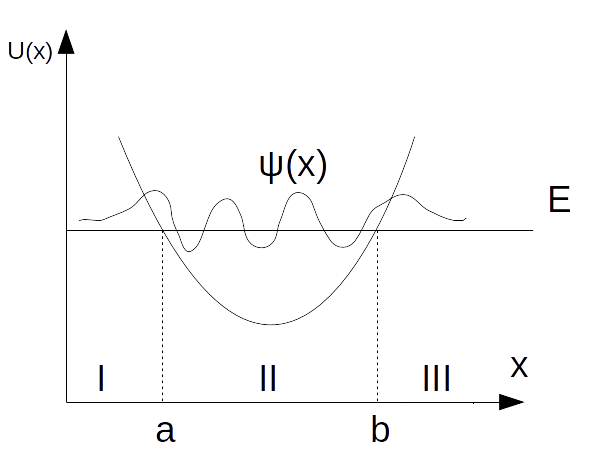
\includegraphics[scale=1]{figs/11_4}
\caption{К выводу условий квантования Бора-Зоммерфельда}
\label{fig:11_4}
\end{figure}

Применим правило соответствия I:
$$
\begin{gathered}
\psi(x)_{x<b} = \frac{a_1}{\sqrt{p}} \sin\brs{\frac{1}{\hbar} \int_{x}^{b} p(x')dx' + \frac{\pi}{4} } \equiv \frac{a_1}{\sqrt{p}} \sin({z_1 + \frac{\pi}{4}}) \\
\psi(x)_{x>a} = \frac{a_2}{\sqrt{p}} \sin\brs{\frac{1}{\hbar} \int_{a}^{x} p(x')dx' + \frac{\pi}{4} } \equiv \frac{a_2}{\sqrt{p}} \sin({z_2 + \frac{\pi}{4}})
\end{gathered}
$$
$$
z_1+z_2 = \frac{1}{\hbar} \int_{a}^{b} p(x')dx' \equiv \frac{1}{\hbar} \int_{a}^{b} p(x)dx
$$
<<Сшивка>> (на интервале $(a, b)$ волновые функции обязаны совпадать):
$$
\begin{aligned}
\frac{a_1}{\sqrt{p}} \sin({z_1+\frac{\pi}{4}}) = \frac{a_2}{\sqrt{p}} \sin({z_2+\frac{\pi}{4}}) = \frac{a_2}{\sqrt{p}} \sin\brs{\frac{1}{\hbar} \int_{a}^{b} p(x)dx - z_1 + \frac{\pi}{4}} = \\
= -\frac{a_2}{\sqrt{p}} \sin\brs{z_1 - \frac{1}{\hbar} \int_{a}^{b} p(x)dx - \frac{\pi}{4} }
\end{aligned}
$$

Условия совпадения решений:
\begin{equation}
\label{eq:11_3_1}
z_1 + \frac{\pi}{4} = z_1 - \frac{1}{\hbar} \int_{a}^{b} p(x)dx - \frac{\pi}{4} + \pi(n+1) \\
\end{equation}
\begin{equation}
\label{eq:11_3_2}
a_1 = (-1)(-1)^{n+1}a_2  ~~\rightarrow~~ a_2 = a_1 (-1)^n
\end{equation}

Отсюда получаем \textbf{условия квантования Бора-Зоммерфильда} (1915-й год):
\begin{equation}
\label{eq:11_3_3}
\boxed{\int_{a}^{b} p(x)dx = \pi\hbar\brc{n+\frac{1}{2}}}
\end{equation}

\begin{equation}
\label{eq:11_3_4}
\boxed{\oint p(x)dx \equiv \int_{a}^{b} p(x)dx = 2\pi\hbar\brc{n+\frac{1}{2}}}
\end{equation}

Напомним:
$$
p(x) = \sqrt{2m(E_n - U(x))}
$$

Выводы:
\begin{enumerate}
\item $\oint p(x)dx $ --- адиабатический инвариант (система сохраняет квантовый уровень при медленном (адиабатическом) изменении параметров системы)
\item $n:~ n \to E_n$
$$
\sin({z+\frac{\pi}{4}}):~~ a \to b:~ \frac{\pi}{4} \to \frac{1}{\hbar} \left. \int_{a}^{b} p(x)dx + \frac{\pi}{4} \right|_{\text{\eqref{eq:11_3_3}}} =
\pi n + \frac{3}{4}\pi
$$
Следовательно, волновая функция на промежутке от $a$ до $b$ меняет знак $n$ раз, что является частным случаем осцилляционной теоремы (гл. 7 \textsection 3)
\end{enumerate}

Малый параметр ВКБ:
$$
\frac{\lambdabar}{L} \sim \frac{1}{n} \ll 1 \sim \frac{1}{2} ~~\rightarrow~~ n >> 1
$$
т.е. условия квантования Бора-Зоммерфильда пригодны при больших $n$ (\textbf{TODO}: почему при этом нельзя опустить $\frac{1}{2}$?)

\section{Фазовый объём, приходящийся на одно квантовое состояние}

Рассмотрим фазовую плоскость $(p,x)$:

$$
\oint p(x)dx = \Gamma(E_n) = 2\pi\hbar\brs{n+\frac{1}{2}}
$$

$$
E_n \to E_{n+1}: \boxed{\Delta\Gamma = \Gamma(E_{n+1}) - \Gamma(E_n) = 2\pi\hbar}
$$
т.е. на одно квантовое состояние в фазовом пространстве частицы приходится объём $2\pi\hbar$

Число квантовых состояний в некотором фазовом объёме:
$$
\boxed{\Delta N = \frac{\Delta p \Delta x}{2\pi\hbar}}
$$

\begin{sloppypar}
  \section{Вероятность проникновения частицы через барьер в квазиклассическом приближении}
\end{sloppypar}

\begin{figure}[h]
\centering
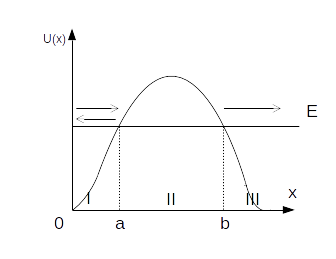
\includegraphics[scale=1]{figs/11_5}
\caption{Проникновение частицы через барьер}
\label{fig:11_5}
\end{figure}


\begin{enumerate}
\item Область III:
$$
\psi(x)_{x>b} \simeq \frac{A}{\sqrt{p(x)}} \exp\brc{\frac{i}{\hbar} \int_{b}^{x} p(x')dx' + i\frac{\pi}{4}}
$$

Проверим, что данная волновая функция действительно соответствует прошедшей волне: найдём плотность потока вероятности:
$$
\begin{aligned}
j_{x}^{\text{прош}} = \frac{i\hbar}{2m}(\psi\nabla\psi^* - \psi^*\nabla\psi) = \brc{\text{члены}~ \sim \nabla \frac{1}{\sqrt{p(x)}} ~\text{компенсируются}} =\\
= \frac{i\hbar}{2m} \brcr{\frac{A}{\sqrt{p(x)}} e^{i\brs{z(x)+\frac{\pi}{4}}} \frac{A^*}{\sqrt{p(x)}} e^{-i\brs{z(x)+\frac{\pi}{4}}} \brc{-i\frac{dz}{dx}} - \brc{\text{компл-сопр}} } = \\
= \frac{i\hbar}{2m} \brcr{\frac{-i\abs{A}^2 2}{\hbar}} = \frac{\abs{A}^2}{m} = j_x^{\text{прош}} > 0
\end{aligned}
$$
т.е. $\psi(x)_{x>b}$ действительно описывает прошедшую волну.

\item Область II, по правилу соответствия III:
$$
\psi(x)_{a<x<b} \simeq \frac{A}{\sqrt{\abs{p}}} \exp\brc{\frac{1}{\hbar} \int_x^{b} \abs{p(x')}dx'} \equiv 
$$
$$
\equiv \frac{A}{\sqrt{\abs{p}}} \underbrace{ \exp\brc{\frac{1}{\hbar} \int_{a}^{b} \abs{p(x')}dx'} }_{e^{\gamma}} \exp\brc{- \frac{1}{\hbar} \int_{a}^{x} \abs{p(x')}dx'}
$$

\item Область I, правило соответствия I:
$$
\psi(x)_{x<a} \simeq \frac{2A}{\sqrt{p}} \sin\brs{\frac{1}{\hbar} \int_{x}^{a} p(x')dx' + \frac{\pi}{4}} e^{\gamma} =
$$
$$
= \frac{2A e^{\gamma}}{\sqrt{p}} \left\{ \underbrace{\exp \brc{\frac{i}{\hbar} \int_{x}^{a} p(x')dx' + \frac{i\pi}{4}}}_{\text{отраженная волна}} - \underbrace{\exp \brc{-\frac{i}{\hbar} \int_{x}^{a} p(x')dx' - \frac{i\pi}{4}}}_{\text{падающая волна}}\right \} 
$$
$$
j_x^{\text{пад}} = \frac{i \hbar}{2m} \brcr{\Psi \nabla \Psi^* - \Psi^* \nabla \Psi} = \frac{i \hbar}{2m} \brcr{\frac{A e^{\gamma}}{i \sqrt{p}} e^{-i(z(x) + \frac{\pi}{4})} \frac{A^* e^{\gamma}}{(-i) \sqrt{p}} e^{i(z(x) + \frac{\pi}{4})} \brc{i \frac{dz}{dx}} - \text{К.С.} } =
$$
$$
= \frac{i \hbar}{2m} \brcr{\frac{-2i \abs{A}^2 e^{2\gamma}}{\hbar}} = \frac{\abs{A}^2 e^{2\gamma}}{m}
$$

\item Формула Гамова (1928г):
$$
\boxed{D \equiv \frac{\abs{j_x^{\text{прош}}}} {\abs{j_x^{\text{пад}}}} = e^{2\gamma} = e^{-\frac{2}{\hbar} \int_a^b \abs{p(x)} dx}} 
$$

Коэффициент отражения:
$$
R \equiv \frac{\abs{j_x^{\text{отр}}}}{\abs{j_x^{\text{пад}}}} = 1 (!)
$$
Это свойство имеет место в квазиклассике, т.к. при установлении правил соответствия растущая экспонента компенсирует падающую экспоненту.

$D \ll 1 \to 2\gamma \ll 1$
\end{enumerate}
>>>>>>> Правки Елены Лимоновой: Исправлена и дополнена Глава 11
